\documentclass[fleqn]{jbook}
\usepackage{graphicx}
\begin{document}

\begin{question}{第1問}{山崎}
次の英文はH.~A. ~Betheの講演からの抜粋である。これを読み以下の設問(i)、(ii)、(iii)、(iv)に答えよ。

\bigskip

\qquad From time immemorial people must have been curious to know what \fbox{(a)} the sun shining. The first scientific attempt at an explanation was by Helmholtz about one hundred years ago, and was based on the force most familiar to physicists at the time, gravitation. When a gram of matter falls to the sun's surface it \fbox{(b)} a potential energy
\begin{equation}
E_{pot}=-GM/R=-1.91\times 10^{15} \textrm{ erg/g},
\end{equation}
where $M=1.99\times 10^{33} \text{ g}$ is the sun's mass, $R=6.96\times 10^{10}\text{ cm}$ its radius, and $G=6.67\times 10^{-8}$ the gravitational constant. A similar energy was set free when the sun was assenbled from interstellar gas or dust in the dim past; actually somewhat more, because most of the sun's material is localted closer to its center, and therefore has a numerically larger potential energy. One-half of the energy set free is \fbox{(c)} into kinetic energy according to the well-known virial theorem of mechanics. This will permit us alter to estimate the temperature in the sun. The other half of the potential energy is radiated away. We have known that at present the sun radiates
\begin{equation}
\epsilon=1.96 \text{ erg/g sec}.
\end{equation}
Therefore, if gravitation supplies the energy, there is enought energy available to supply the radiation for about $10^{15}$ sec which is about 30 million years.

\qquad This was long enough for nineteenth century physicists, and certainly a great deal longer than man's recorded history. It was not long enough for the biologists of the time. Darwin's theory of evolution had just become popular, and biologists argued with Helmholtz that evolution would require a longer time than 30 million years, and that therefore his energy source for the sun was insufficient. They were right.

\qquad $_{(1)}$\underlinedtext{At the end of the 19th century, radioactivity was discovered by Becquerel and the two Curie's who received one of the first Nobel prizes for this discovery. Radioactivity permitted a determination of the age of the earth, and more recently, of meteorites which indiate the time at which matter in the solar system solidified. On the bases of such measurements the age of the sun is estimated to be 5 milliards of years, within about 10 \%. So gravitation is not sufficient to supply its energy over the ages.}

\qquad Eddington, in the 1920's, investigated very thorougly the interior constitution of the sun and other stars, and was much concerned about the sources of stellar energy. His favorite hypothesis was the complete annihilation of matter, changing nuclei and electrons into radiation. The energy which was to be set free by sucha process, if it could \fbox{(d)}, is given the by $_{(2)}$\underlinedtext{the Einstein relation} between mass and energy and is
\begin{equation}
c^2=9\times 10^{30} \text{erg/g}
\end{equation}
This would be enough to \fbox{(e)} the sun's radiation for 1500 milliards of years. However nobody has ever observed the complete annihilation of matter. From experiments on earth we know that protons and electrons do not annihilated each other in $10^{30}$ years. It is hard to believe that the situation would be different aa a temperature of some 10 million degrees such as \fbox{(f)} in the stars, and Eddington appreciated this difficulty quite well.


\qquad $_{(3)}$\underlinedtext{From the early 1930's it was generally assumed that the stellar energy is produced by nuclear reactions. Already in 1929, Atkinson and Houtermans concluded that at the high temperatures in the interior of a star, the nuclei in the star could penetrate into other neclei and cause nuclear reactions, releasing energy. In 1933, particle accelerators began to operate in which such nulcear reactions were actually observed.} They were found to obey very closely the theory of Gamow, Condon and Gurney, on the penetration of charged particles throug potential barrirers. In early 1938, Gamow and Teller revised the theory of Atkinson and Houtermans on the rate of $\ll$ themonuclear $\gg$ reations, i.e. nuclear reactions occurring at high temperature. At the same time, von Weizs\"acker speculated on the reactions which actually might take place in the stars.

\hspace{1cm} meteorite: 隕石. \\
\hspace{1cm} 1 erg=$10^{-7}$ J (cgs単位). \\
\hspace{1cm} milliard: 10億. \\

%\begin{enumerate}
%\renewcommand{\labelenumi}{(\roman{enumi})}
(i)文章中の(a)から(f)まで6箇所の四角にあてはまる単語の原型を次の中からえらべ。

(ア)transform(イ)supply(ウ)keep(エ)get(オ)prevail(カ)occur

\begin{table}[htbp]
\begin{center}
\begin{tabular}{|c|c|c|c|c|c|c|c|c|c|c|c|}
\hline
(a) &   & (b) &   & (c) &   & (d) &   & (e) &   & (f) &   \\
\hline
\end{tabular}
\end{center}
\end{table}


(ii) 下線部(1)を和訳せよ。\\

(iii) 下線部(2)のthe Einstein relationとはなんであるか、簡単に英語で説明せよ。\\

(iv) 下線部(3)を和訳せよ。\\
%\end{enumerate}
\end{question}

\begin{answer}{第1問}{}
(i)
\begin{table}[h]
\begin{center}
\begin{tabular}{|c|c|c|c|c|c|c|c|c|c|c|c|}
\hline
(a) &  ウ  & (b) &  エ  & (c) &  ア  & (d) &  カ  & (e) &  イ  & (f) &  オ  \\
\hline
\end{tabular}
\end{center}
\end{table}
\\
(ii)\\
 19世紀末、ベクレルと二人のキューリーによって放射能が発見され、彼らはこの発見により初期のノーベル賞を受賞した。放射能は地球の年齢の決定を可能にし、さらに最近では、太陽系で物質が凝固した年代を暗示する隕石の年齢の決定も可能にした。このような測定に基づくと太陽の年齢は、10%以内の誤差で、50億年であると見積もられる。よって重力は、このような長い年月もの間太陽のエネルギーを供給するには不十分である。\\
\\
(iii)\\
 The Einstein relation between mass and energy contends that mass and energy are equivalent. Their relation is given by the equation "$\epsilon ^2 = mc^2$" , where $\epsilon $ represents the energy, $m$ the mass, and $c$ the speed of the light.\\
\\
(iv)\\
 1930年代初頭より、星のエネルギーは核反応によって生み出されているのだと一般的に考えられるようになった。1929年にすでに、アトキンソンとホーターマンが、星の中心の高い温度においては星の中の原子核は他の原子核まで到達することができ、エネルギーの解放をともなう核反応を起こすことができると結論したのだ。1933年には、このような核反応が実際に観測されるような粒子加速器が稼動しはじめた。\\


\end{answer}


\begin{question}{第2問}{}
次の英文はR.~A.~Millikanの講演からの抜粋である。これを読み以下の設問(i),(ii),(iii)に答えよ。

\bigskip

\qquad The most direct and unambiguous proof of the existence of the electron will probably be generally admitted to be found in an experiment which for convenience I will call the oil-drop experiment. But before discussing the significance of that advance I must ask you to bear with me while I give the experimentalist's answer to the very fundamental but bery familiar query: $\ll$ What is electricity? $\gg$ His answer is naive, but simple and definite. He admits at once that as to the ultimate nature of electricity he knows nothing.

\qquad He begins rather with a few simple and familiar experiments and then sets up some definitions which are only descriptions of the experiments and therefore involve no hypothetical elements at all.

\qquad He first notes the fact that a pith ball, after contact with a glass rod that has been rubbed with silk, is found to be endowed with the new and striking property that it tends to move away from the rod with a surprisingly strong and easily measurable force. He describes that facet, and affirms at the same time his ignorance of all save the existence of this force, by inventing a new word and saying that the pith ball bas been put into a positively electrified state, or simplly has received a charge of positive electricity. He then measures the amount of its charge by the strength of the observed force.

\qquad Similarly he finds that the pith ball, after contact with an ebonite rod that has been rubbed with cat's fur is attracted, and he proceeds to describe this experiment by sayign that it has now received a charge of negative electriciy. Whenever the pith ball is found to have been put, by contact with any body or by any other process, into a condition to behave in either of the foregoing ways, it has, by definitions, received a charge of either positive of negative electricity. The whole of our thinking about electrical matters starts with these two simple experiments and those two definitions.

\qquad In order now to get the most crucial possible test of the correctness of incorrectness of Franklin's conception of a particle, or an atom, of electricity it was clearly necessary to reduce the charge on the pith ball to the smallest possible amount, to change that charge by the most minute possible steps, and then to se whether the forces acting upon it at a given distance from the glass rod (i.e. in a constant field) had any tendency to increase or decrease by unitary steps.

\qquad The success of the experiments first performed in 1909, was wholly due to the design of the apparatus, i.e. to the relation of the parts.

\qquad The pith ball itself which was to take on the smallest possible charge had of course to be the smallest spherical body which could be found and yet which would remain of constant mass; for a continuously changing gravitational force would be indistinguishable, in its effect upon the motion of the charged body, from a continously chaning electrical charge.

\qquad A non-homogeneous or no-spherical body also could not be tolerated; for the force acting on the pith ball had to be measured by the speed of mation imparted to it by the field, and this force could not be computed from the speed unless the shape ws spherical and the density absolutely constant. This is why the body chosen to replace the pith ball was an individual oil-droplet about a thousandth of a milimeter in diamter blown out of an ordinary atomizer and kept in an atmosphere from which convection currents had been completely removed by suitable thermostatic arrangements. The glass rod, the purpose of which as to produce a constant electrical field, was of course replaced by the two metal plates C and D (Dif.1 ) of an air condenser, one of the plates (D) being attached to the positive, the other (C) to the negative termial of a battery, and aswitch beging added, as shown in the figure, so as to make it possible to throw the field on or off at will.

\hspace{1cm} pith: 木髄、植物の茎の中心にある柔らかい組織、軽く、帯電しやすい性質を持つ。\\
\hspace{1cm} rod: 棒.~~save: を除いて(=except).\\
\hspace{1cm} spherical: 球形の.~~atomizer: 噴霧器.\\
\hspace{1cm} convection currents: 対流\\

%\begin{enumerate}
%\renewcommand{\labelenumi}{(\roman{enumi})}
(i)
Millikanは木髄球が受け取った電荷が正であるか、あるいは負であるかを調べるためには、どのような実験を行えば良いと言っているのだろうか。それぞれの場合の木髄球の振る舞いも答えよ。\\

(ii)
油滴の落下実験を成功に導いた油滴の特徴について、本文中に述べられていることを箇条書きにしてすべて挙げよ。\\

(iii)ここには示していないが、原文では実験装置の概略図(Fig. 1)が描かれている。その一部である2枚の金属板(CとD)を含む回路図を、本文中の説明をもとに描け。\\
\end{question}

\begin{answer}{第2問}{}
(i)\\
 木髄球に絹でこすったガラス棒を近づけて、木髄球の動きを見れば良いと言っている。もし木髄球が正に帯電しているならガラス棒から離れようとし、逆に負に帯電しているならガラス棒に引き寄せられる。\\
\\
(ii)
\begin{itemize}
\item 最小の電荷を受け取れるように、油滴が、実現できる最小の大きさであったこと。
\item 電場から受ける力を計算できるように、油滴が球型であったこと。
\item 油滴の質量が同じになるように、質量密度が完全に一定であったこと。
\end{itemize}
 \\
(iii)
\begin{figure}[h]
\vspace*{-\intextsep}
 \begin{center}
  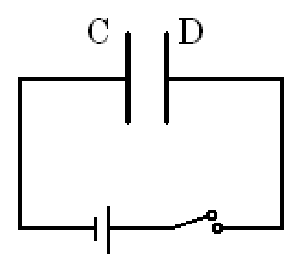
\includegraphics{2004engl2-1.eps}
 \end{center}
\end{figure}
\end{answer}

\end{document}